\documentclass[main]{subfiles}
\begin{document}
\chapter{简介}\label{chp:intro}

子空间聚类问题来自于很多实际的应用,包括运动轨迹分离~\cite{costeira1998motion_seg},
人脸识别~\cite{basri2003lambertianface},网络跳点计数~\cite{eriksson2011high_rankMC},
电影评分~\cite{zhang2012RecSys} 以及社交图谱~\cite{xu2011graphclustering}。
这些应用产生的高维数据通常可以看作是从多个混合的低维线性子空间的采样(如图\ref{fig:Union_of_sub_model}所示)。
子空间聚类就是在不知道类别信息的情况下,将这些数据按照它们原本所属的子空间重新聚合,
并且恢复出数据中隐含的子空间结构。
对应于上面所述的应用,子空间聚类能根据运动轨迹分离刚体,判断哪些面部照片来自同一个人,哪些网络
节点属于一个子网,给出观影兴趣相似的用户以及发现社交网络中隐含的人际关系。

\begin{figure}
  \centering
  % Requires \usepackage{graphicx}
  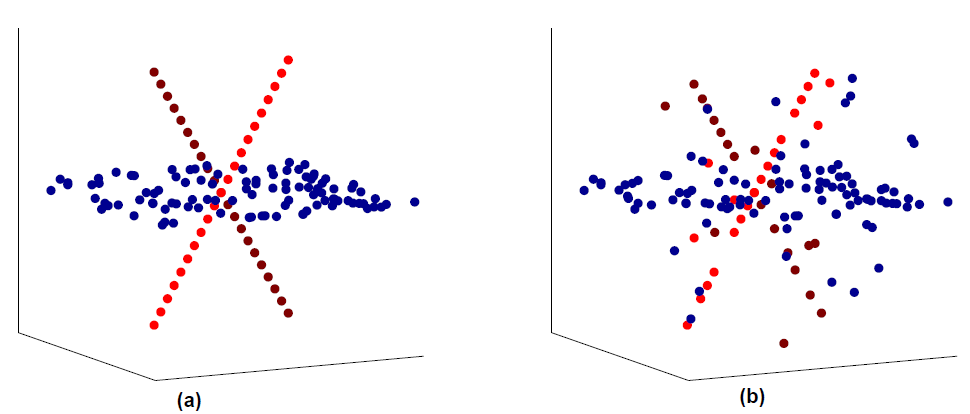
\includegraphics[width=0.8\linewidth]{pics/Union_of_Subspace.png}\\
  \caption{采样于三个子空间的无噪音 (a) 和有噪音 (b) 数据}\label{fig:Union_of_sub_model}
\end{figure}

过去十年,很多人关注子空间聚类问题,并且提出了许多算法,包括 Expectation-Maximization 类型的局部优化算法,
比如 K-plane~\cite{bradley2000k-plane} 和 Q-flat~\cite{tseng2000qflat},代数方法,比如
广义主成分分析(Generalized Principal Component Analysis)~\cite{vidal2005gpca},
矩阵分解方法~\cite{costeira1998motion_seg,costeira2000multibody_factorization},基于谱聚类的方法
~\cite{lauer2009spectral,chen2009spectral},自底向上的局部采样方法~\cite{yan2006LSA,rao2008motion},
以及基于凸优化的方法,比如低秩表示(Low Rank Representation)~\cite{liu2010lrr_icml,liu2013LRR}
和稀疏子空间聚类(Sparse Subspace Clustering)~\cite{elhamifar2009ssc,elhamifar2012ssc_journal}。
这些算法中,SSC是最优秀的之一,尤其当数据有噪音时,表现地相对稳健和鲁棒,例如在运动分割领域的
Hopkins155~\cite{tron2007benchmark,elhamifar2009ssc}测试集上,SSC是目前公认的表现最好的算法,
并且当类别增多时,它表现得比 LRR 更好~\cite{elhamifar2012ssc_journal}。

SSC算法的关键是将每个数据点用其他点线性表示,由于每个点都在一个低维子空间中,则一定存在一个相对稀疏的表示,
只用到同一个子空间中的点。如果把系数大小看作两个点的连接权重,我们可以得到一个无向图,再对这个图进行谱聚类,
即可将不同子空间的点分开。如果用第~\ref{chp:prob_setup}节中的符号描述,那么无噪音和有噪音的 SSC 分别求解
\begin{align*}
  \min_{c_i} \|c_i\|_1\quad s.t.\quad X_i=X_{\{i\}^c}c_i, \\
  \min_{c_i} \|c_i\|_1+\frac{\lambda}{2}\|X_i-X_{\{i\}^c}c_i\|^2,
\end{align*}
$X_i$ 表示数据矩阵的第$i$ 列, $c_i$ 是$X_i$ 用其他所有点表示的系数,我们希望其非零元素对应的数据点都和 $x_i$ 在同一个子空间。
对于仿射子空间,SSC 同样适用,只需要加上 $c_i = i$的限制。

\begin{algorithm}[tb]
  \caption{Sparse Subspace Clustering}
  \label{alg:SSC}
  \begin{algorithmic}
    \State {\bfseries Input:}
    Data points as columns in $X\in \mathbb{R}^{n\times N}$.
    \State{1. } For each data point $x_i$, solve
    \begin{align}\label{eq:SSC}
      \min_{c_i} \; \|c_i\|_1 \quad s.t. \quad &x_i=X_{-i}c_i
    \end{align}
    \State{2. } Let $C:=[c_1,...,c_N]$. Form affinity graph $G$ that is represented by adjacency matrix $W=|C|+|C|^T$.
    \State{3. } Estimate the number of subspace by finding the largest eigenvalue gap of normalized Laplacian of $G$ via
    $$\hat{L}=N-\underset{i=1,...,N-1}{\text{argmax}}\; \sigma_i-\sigma_{i+1}$$
    \State{4. } 对 $G$ using $\hat{L}$.
    \State {\bfseries Output:} Subspace partitions $\mathcal{X}_1,...,\mathcal{X}_{\hat{L}}$
  \end{algorithmic}
\end{algorithm}

然而,在 SSC 中,我们每次只考虑一个点相对于其他点的表示,
比较容易受到噪音和异常点的干扰。如果我们预先知道点$A,B,C$
属于同一类,然后寻找其他几个点能同时表示$A,B,C$,这无疑比
单独考虑$A$ 或 $B$ 或 $C$ 更稳健。另一方面,在SSC 模型中,
我们只是要求稀疏尽量稀疏,如此产生的邻接矩阵,不一定能在
接下来的谱聚类中有比较好的可分性。如果我们能让表示向量的非零元
集中在某些位置,那么邻接矩阵将具有更好的结构(具体可见第\ref{chp:experiments}节)

基于上面的考虑,本文结合了压缩感知中的 joint sparse 模型\cite{}, 提出了一种新的子空间聚类方法,它的核心内容有两步:
第一步是根据点的空间信息,先将某些点聚在一起,组成若干组。第二部有两种方法,
可以把一组的点作为整体,相对其他店做回归,要求他们同时被稀疏表示,这是
\bf{Multitasking 方法},也可以依然像SSC那样,把一个点用其他点表示,但是
采用类似于Group LASSO的优化范数。同样地得到表示系数,进而构造邻接矩阵。

\end{document}
